\chapter{Statika Fluida}\label{ch:b1:fluid-statics}

Sebuah kapal selam pada kedalaman tiga ratus meter mengemban, pada tiap meter
persegi lambungnya, berat sebuah truk bermuatan. Sebuah bendungan menahan danau dengan
dinding yang tebal di bawah dan tipis di atas, karena alasan
yang sama sekali tak berhubungan dengan panjang danaunya. Sebuah kapal seratus
ribu ton terapung karena ia menyisihkan seratus ribu ton
air, dan tenggelam sejengkal lebih dalam ketika ia berlayar dari laut
masuk ke sungai. Setiap satu di antaranya adalah akibat satu hubungan tunggal
--- tekanan bertambah ke bawah dalam fluida yang diam dengan laju $\rho g$ ---
dan bab ini menurunkannya, menerapkannya pada zat cair dan atmosfer,
lalu menyimpulkan darinya gaya pada sebuah dinding dan hukum Archimedes.

\begin{omfigure}
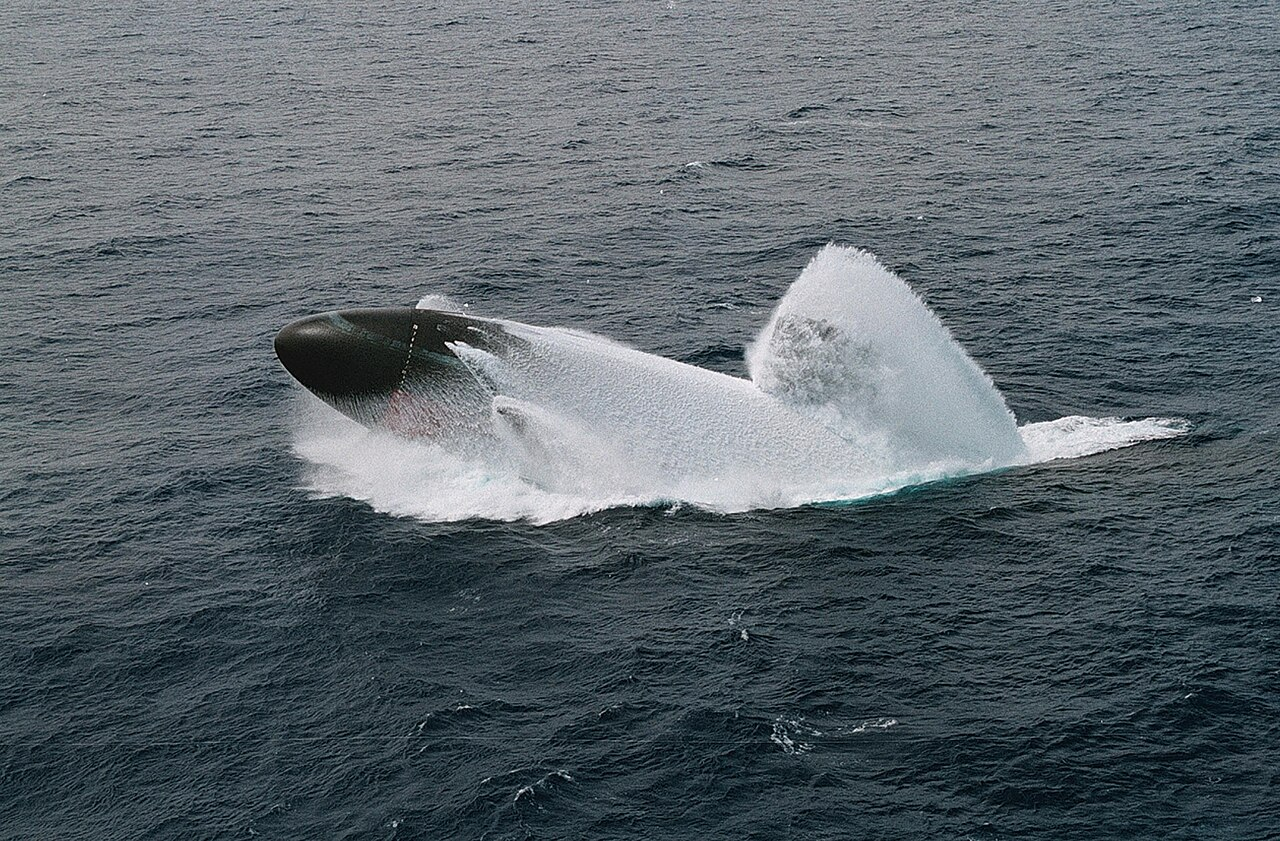
\includegraphics[width=0.60\linewidth]{images/book3/submarine-surfacing.jpg}

{\small Sebuah kapal selam dalam latihan muncul darurat (Angkatan Laut Amerika Serikat): tangki pemberatnya dikosongkan, ia menjadi lebih ringan daripada air yang didesaknya lalu naik --- teorema Archimedes pada \qty{7000}{t}.}
\end{omfigure}

\section{Tekanan dalam fluida yang diam}

\begin{proposition}[Keisotropikan tekanan]\label{prop:b1:fluid-statics:isotropy}
\index{tekanan!dalam fluida}
Dalam fluida yang diam, gaya yang dikerahkan fluidanya pada permukaan kecil
$\dd S$ yang diletakkan di titik $M$ adalah $\dd\vect F = P(M)\,\dd S\,\vect n$, tegak lurus pada
permukaannya dan terarah menujunya, dengan tekanan $P(M)$ yang bergantung
pada titiknya tetapi \emph{tidak} pada arah hadap permukaannya.
\end{proposition}

\begin{proof}[Bukti sebagian]
Fluida yang diam tak meneruskan gaya tangensial (kalau tidak, ia akan mengalir):
gayanya tegak lurus. Tinjaulah sebuah prisma segitiga fluida yang amat kecil di $M$
dengan muka-muka berarah berbeda: ia setimbang di bawah
gaya tekanan pada muka-mukanya dan beratnya; beratnya berskala sebagai
volumenya (pangkat tiga ukurannya), gaya tekanannya sebagai luas (pangkat
dua), sehingga bagi prisma yang cukup kecil hanya gaya tekanannya yang berperan, dan
keseimbangannya ke segala arah menuntut $P$ yang sama pada tiap muka.
\end{proof}

\begin{theorem}[Hubungan dasar statika fluida]\label{thm:b1:fluid-statics:fundamental}
\index{hubungan hidrostatik}
Dalam fluida yang diam di dalam gravitasi seragam $\vect g = -g\vect e_z$ ($z$
ke atas), tekanannya hanya bergantung pada $z$ dan
\[
\frac{\dd P}{\dd z} = -\rho g ,
\]
dengan $\rho$ massa jenis fluidanya pada aras itu. Tekanan bertambah
ke bawah; permukaan bertekanan sama (\emph{isobar}) mendatar,
demikian pula permukaan bebas sebuah zat cair.
\end{theorem}

\begin{proof}
Ambil sebuah lempeng fluida mendatar seluas $S$ di antara $z$ dan $z + \dd z$:
ia didorong ke atas oleh $P(z)S$ dari bawah, ke bawah oleh $P(z + \dd z)S$ dari atas,
dan ditarik ke bawah oleh beratnya $\rho gS\,\dd z$. Dalam keadaan diam:
$P(z)S - P(z + \dd z)S - \rho gS\,\dd z = 0$. Lempeng fluida mendatar
tak mendapat gaya mendatar dari gravitasi, sehingga secara mendatar $P$ seragam.
\end{proof}

\begin{omfigure}
\begin{tikzpicture}[font=\small, x=1cm, y=1cm]
  \fill[omDef!10] (-2.4,-1.8) rectangle (2.4,1.8);
  \draw[thick, fill=omDef!30] (-1.2,-0.25) rectangle (1.2,0.25);
  \draw[-Stealth, omThm, very thick] (0,-1.3) -- (0,-0.3) node[pos=0.0, below] {$P(z)\,S$};
  \draw[-Stealth, omThm, very thick] (0,1.3) -- (0,0.3) node[pos=0.0, above] {$P(z + \dd z)\,S$};
  \draw[-Stealth, omProp, very thick] (0.9,0) -- (0.9,-0.9) node[right] {$\rho gS\,\dd z$};
  \draw[Stealth-Stealth] (-1.5,-0.25) -- (-1.5,0.25) node[midway, left] {$\dd z$};
  \draw[-Stealth] (2.8,-1.5) -- (2.8,1.5) node[above] {$z$};
  \node[font=\footnotesize] at (0,-2.1) {$P(z) - P(z + \dd z) = \rho g\,\dd z$};
\end{tikzpicture}\qquad
\begin{tikzpicture}[font=\small, x=1cm, y=1cm]
  % communicating vessels
  \fill[omDef!25] (0,0) rectangle (0.8,2.4); \fill[omDef!25] (0,0) rectangle (4.2,0.6); \fill[omDef!25] (1.8,0) rectangle (2.4,2.4); \fill[omDef!25] (3.4,0) rectangle (4.2,2.4);
  \draw[thick] (0,3.2) -- (0,0) -- (4.2,0) -- (4.2,3.2); \draw[thick] (0.8,3.2) -- (0.8,0.6) -- (1.8,0.6) -- (1.8,3.2); \draw[thick] (2.4,3.2) -- (2.4,0.6) -- (3.4,0.6) -- (3.4,3.2);
  \draw[omDef, thick] (0,2.4) -- (0.8,2.4); \draw[omDef, thick] (1.8,2.4) -- (2.4,2.4); \draw[omDef, thick] (3.4,2.4) -- (4.2,2.4);
  \draw[dashed, omThm] (-0.3,2.4) -- (4.5,2.4); \node[omThm, right] at (4.5,2.4) {aras yang sama};
  \node[font=\footnotesize] at (2.1,-0.4) {$P$ yang sama pada satu garis mendatar};
\end{tikzpicture}

{\small Kiri: kesetimbangan sebuah lempeng fluida mendatar --- tekanan
di bawahnya harus melampaui tekanan di atasnya sebesar berat lempengnya tiap satuan luas.
Kanan: bejana berhubungan --- sebuah garis mendatar menemui tekanan
yang sama di mana pun dalam zat cair yang terhubung, sehingga permukaan bebasnya berdiri
pada satu aras berapa pun bentuknya.}
\end{omfigure}

\begin{corollary}[Fluida tak termampatkan]\label{cor:b1:fluid-statics:incompressible}
\index{tekanan hidrostatik}
Dalam zat cair bermassa jenis seragam $\rho$, tekanan pada kedalaman $h$ di bawah
sebuah titik yang tekanannya $P_0$ adalah
\[
P = P_0 + \rho gh .
\]
Air: \qty{1}{bar} lebih besar tiap \qty{10}{m}. Dua titik zat cair terhubung
pada aras yang sama bertekanan sama; permukaan bebas
bejana berhubungan berdiri pada satu aras; tekanan yang dikenakan di mana pun
pada zat cair terkurung diteruskan tanpa berkurang ke setiap titiknya
(asas Pascal).
\end{corollary}

\begin{proof}
Integralkan $\dd P/\dd z = -\rho g$ dengan $\rho$ tetap; sisanya adalah
kemendataran isobar dan ketunggalan $P$ pada satu aras.
\end{proof}

\begin{example}[Manometer dan kempa]\label{ex:b1:fluid-statics:manometer}
\index{manometer}\index{kempa hidraulik}
Sebuah tabung U berisi raksa ($\rho = \qty{13600}{kg/m^3}$) yang selisih tinggi kolomnya
$h = \qty{760}{mm}$ mengukur beda tekanan $\rho gh = \qty{1.013e5}{Pa}$
--- yaitu atmosfer, yang menahan kolom air setinggi \qty{10.3}{m}. Sebuah
\omterm{ex:b1:fluid-statics:manometer}{kempa hidraulik}: gaya $F_1$ pada torak seluas $S_1$ menaikkan
tekanannya sebesar $F_1/S_1$ di mana-mana; pada torak besar $S_2$ ia menghasilkan
$F_2 = F_1S_2/S_1$ --- lima puluh kali lebih besar untuk luas lima puluh kali lipat, dengan
harga jarak tempuh lima puluh kali lebih pendek (energinya kekal: $F_1d_1 = F_2d_2$).
\end{example}

\section{Atmosfer}

\begin{proposition}[Atmosfer isotermal]\label{prop:b1:fluid-statics:atmosphere}
\index{rumus barometrik}\index{tinggi skala}
Bagi \omterm{def:b1:kinetic-theory:model}{gas ideal} bermassa molar $M$ pada suhu seragam $T$ di dalam gravitasi
yang seragam,
\[
P(z) = P_0\,\eu^{-z/H}, \qquad H = \frac{RT}{Mg} ,
\]
itulah \emph{\omterm{prop:b1:fluid-statics:atmosphere}{tinggi skala}}: kira-kira \qty{8}{km} untuk udara; tekanannya menjadi separuh
tiap $H\ln2 \approx \qty{5.5}{km}$.
\end{proposition}

\begin{proof}
$\rho = PM/RT$ (persamaan keadaan), sehingga $\dd P/\dd z = -(Mg/RT)P$: sebuah
persamaan linear orde satu, $P = P_0\eu^{-Mgz/RT}$.
\end{proof}

\begin{example}[Udara tipis]\label{ex:b1:fluid-statics:altitude}
Dengan $T = \qty{260}{K}$ (rata-rata atas atmosfer bawah), $H =
\qty{7.6}{km}$: $P = 0.52P_0$ pada \qty{5000}{m}, $0.31P_0$ di puncak
Everest --- dekat dengan hasil ukur $0.54$ dan $0.33$; atmosfer yang sebenarnya
mendingin terhadap ketinggian, dan volume Tahun ke-2 memperhitungkannya. Model
ini juga memberitahukan mengapa laut berbeda: air delapan ratus kali lebih
padat dan hampir tak termampatkan, sehingga tekanannya naik secara linear, satu bar
tiap sepuluh meter, tanpa \omterm{prop:b1:fluid-statics:atmosphere}{tinggi skala}.
\end{example}

\begin{omfigure}
\begin{tikzpicture}
\begin{axis}[omaxis, axis x line=bottom, axis y line=left, width=8cm, height=5.4cm, xlabel={$z$ (\unit{km})}, ylabel={$P/P_0$},
    xlabel style={at={(axis description cs:0.5,-0.12)}, anchor=north},
    xmin=0, xmax=30, ymin=0, ymax=1.1, xtick={5.5,10,20,30}, xticklabels={$5.5$,$10$,$20$,$30$}, ytick={0.5,1}]
  \addplot[omDef, thick, domain=0:30, samples=100] {exp(-x/7.6)};
  \draw[dashed, omExo] (axis cs:0,0.5) -- (axis cs:5.3,0.5) -- (axis cs:5.3,0);
  \node[omDef, font=\footnotesize] at (axis cs:16,0.45) {$P_0\eu^{-z/H}$, $H = \qty{7.6}{km}$};
\end{axis}
\end{tikzpicture}

{\small Atmosfer isotermal: tekanan (dan massa jenisnya) turun
secara eksponensial terhadap ketinggian, menjadi separuh tiap \qty{5.5}{km}. Sembilan persepuluh
udaranya terletak di bawah \qty{17}{km}.}
\end{omfigure}

\section{Gaya pada dinding}

\begin{proposition}[Gaya pada dinding tegak]\label{prop:b1:fluid-statics:wall}
\index{pusat tekanan}
Zat cair sedalam $h$ yang menekan dinding persegi panjang tegak selebar $L$
(tekanan atmosfer bekerja pada kedua mukanya dan saling meniadakan) mengerahkan
gaya mendatar
\[
F = \tfrac12\rho gh^2L ,
\]
yang setara dengan sebuah gaya tunggal yang bekerja di \emph{\omterm{prop:b1:fluid-statics:wall}{pusat tekanan}},
pada kedalaman $2h/3$ --- resultannya bekerja di bawah, tempat tekanannya
terbesar.
\end{proposition}

\begin{proof}
Pada kedalaman $x$ tekanan toloknya $\rho gx$; pada jalur setinggi
$\dd x$ gayanya $\rho gxL\,\dd x$; integralkan dari $0$ sampai $h$. Momennya
terhadap garis permukaannya adalah $\int_0^h\rho gx^2L\,\dd x = \tfrac13\rho gh^3L$;
membaginya dengan $F$ memberikan \omterm{def:b1:angular-momentum:moment}{lengan gaya} $2h/3$.
\end{proof}

\begin{omfigure}
\begin{tikzpicture}[font=\small, x=1cm, y=1cm]
  \fill[omDef!20] (-3.6,0) rectangle (0,2.8);
  \draw[thick] (-3.8,2.8) -- (0,2.8); \draw[omDef, thick] (-3.6,2.8) -- (0,2.8);
  \draw[thick, fill=omExo!40] (0,0) -- (0,3.2) -- (1.0,3.2) -- (1.8,0) -- cycle;
  \draw[thick] (-3.8,0) -- (2.6,0);
  \foreach \y/\l in {2.5/0.15, 2.0/0.4, 1.5/0.65, 1.0/0.9, 0.5/1.15, 0.1/1.35} {\draw[-Stealth, omThm] (-\l,\y) -- (0,\y);}
  \draw[omThm, dashed] (0,2.8) -- (-1.4,0);
  \draw[-Stealth, omThm, very thick] (-2.6,0.93) -- (-0.05,0.93) node[pos=0.0, left] {$F = \tfrac12\rho gh^2L$};
  \draw[Stealth-Stealth] (2.2,2.8) -- (2.2,0.93) node[midway, right] {$\tfrac23 h$};
  \draw[Stealth-Stealth] (-3.2,2.8) -- (-3.2,0) node[midway, left] {$h$};
\end{tikzpicture}

{\small Tekanan pada sebuah bendungan tumbuh linear terhadap kedalaman (anak panah), sehingga
resultannya bekerja pada dua pertiga kedalamannya: dindingnya harus paling tebal di
dasarnya. Gayanya bergantung pada $h$ dan $L$, bukan pada berapa banyak air
yang berada di belakangnya.}
\end{omfigure}

\begin{example}[Sebuah bendungan]\label{ex:b1:fluid-statics:dam}
$h = \qty{20}{m}$, $L = \qty{100}{m}$: $F = \tfrac12 \times 1000 \times 9.81 \times
400 \times 100 = \qty{2.0e8}{N}$ --- dua puluh ribu ton, yang bekerja
\qty{13}{m} di bawah permukaannya, sama saja apakah danau di belakangnya sebuah kolam
atau sebuah fyord: itulah \emph{paradoks hidrostatik}.
\end{example}

\section{Teorema Archimedes}

\begin{theorem}[Archimedes]\label{thm:b1:fluid-statics:archimedes}
\index{teorema Archimedes}\index{gaya apung}\index{pusat apung}
Sebuah benda yang terendam dalam fluida yang diam menerima dari gaya tekanannya sebuah
resultan --- yaitu \emph{\omterm{thm:b1:fluid-statics:archimedes}{gaya apung}} --- yang sama besar dan berlawanan dengan berat
fluida yang didesaknya,
\[
\vect\Pi = -\rho_{\text{fluida}}V_{\text{tercelup}}\,\vect g ,
\]
yang bekerja di \omterm{def:b1:systems-of-points:cm}{pusat massa} fluida yang didesaknya (yaitu \emph{\omterm{thm:b1:fluid-statics:archimedes}{pusat apung}}).
\end{theorem}

\begin{proof}
Gaya tekanan pada permukaan bendanya hanya bergantung pada bentuk
permukaan itu dan pada fluida di luarnya. Gantilah bendanya, dalam pikiran, dengan
fluida yang diam yang mengisi volume yang sama: fluida itu setimbang
di bawah beratnya dan gaya tekanan yang sama, sehingga gaya tekanannya
mengimbangi beratnya --- jumlahnya $-\rho V\vect g$, yang bekerja melalui
\omterm{def:b1:systems-of-points:cm}{pusat massanya}. Batalkan percobaan pikirannya; gaya tekanannya tak
berubah.
\end{proof}

\begin{corollary}[Terapung]\label{cor:b1:fluid-statics:floating}
\index{terapung}
Sebuah benda bermassa jenis $\rho_b$ terapung dalam fluida bermassa jenis $\rho_f > \rho_b$
dengan pecahan $\rho_b/\rho_f$ volumenya tercelup; bila $\rho_b >
\rho_f$ ia tenggelam, dengan berat semu $(\rho_b - \rho_f)Vg$.
\end{corollary}

\begin{proof}
Berat $\rho_bVg$ sama dengan \omterm{thm:b1:fluid-statics:archimedes}{gaya apung} $\rho_fV_{\text{terc}}g$.
\end{proof}

\begin{omfigure}
\begin{tikzpicture}[font=\small, x=1cm, y=1cm]
  \fill[omDef!15] (-3.6,-2.2) rectangle (3.6,0);
  \draw[omDef, thick] (-3.6,0) -- (3.6,0);
  % iceberg-like block: rectangle 2 x 1.6, 90% immersed
  \draw[thick, fill=white] (-1.0,-1.44) rectangle (1.0,0.16);
  \fill (0,-0.64) circle (1.5pt) node[right] {$G$};
  \fill[omDef] (0,-0.72) circle (1.5pt) node[left] {$C$};
  \draw[-Stealth, omThm, very thick] (0,-0.64) -- (0,-1.9) node[below] {$\rho_bVg$};
  \draw[-Stealth, omDef, very thick] (0,-0.72) -- (0,0.55) node[above] {$\rho_fV_{\text{terc}}g$};
  \node[font=\footnotesize] at (2.4,-1.2) {$\dfrac{V_{\text{terc}}}{V} = \dfrac{\rho_b}{\rho_f}$};
\end{tikzpicture}

{\small Sebuah benda terapung: beratnya, yang bekerja di \omterm{def:b1:systems-of-points:cm}{pusat massanya} $G$,
mengimbangi \omterm{thm:b1:fluid-statics:archimedes}{gaya apungnya}, yang bekerja di \omterm{thm:b1:fluid-statics:archimedes}{pusat apungnya} $C$ (yaitu
pusat volume yang tercelup). Es ($\rho = \qty{917}{kg/m^3}$) di dalam air
laut ($\qty{1025}{kg/m^3}$): $89\%$ di bawah permukaannya.}
\end{omfigure}

\begin{example}[Tiga gaya apung]\label{ex:b1:fluid-statics:buoy}
Sebuah hidrometer adalah tabung berpemberat yang tenggelam sampai ia mendesak
beratnya sendiri: makin padat zat cairnya, makin dangkal ia tenggelam --- sebuah pengukur massa jenis yang dibaca
pada batangnya. Sebuah balon \qty{2800}{m^3} berisi udara panas pada \qty{373}{K} mendesak
\qty{3.4}{t} udara dingin dan berbobot \qty{2.6}{t} udara panas: \qty{0.7}{t}
daya angkat (\cref{pb:b1:kinetic-theory:1}). Sebuah kapal \qty{100000}{t}
mendesak \qty{97600}{m^3} air laut; di air tawar ($\qty{1000}{kg/m^3}$)
ia harus mendesak $2.5\%$ lebih banyak dan tenggelam lebih dalam --- itulah tanda Plimsoll pada
lambungnya.
\end{example}

\begin{remark}[Kemantapan]\label{rem:b1:fluid-statics:stability}
\index{metasentrum}
Sebuah benda terapung yang dimiringkan sedikit akan dipulihkan bila \omterm{thm:b1:fluid-statics:archimedes}{gaya apungnya},
yang kini bekerja di pusat volume tercelup yang baru dan bergeser, menghasilkan
momen pemulih --- dan itu terjadi bila \emph{metasentrum} (yaitu titik
tempat garis kerja \omterm{thm:b1:fluid-statics:archimedes}{gaya apungnya} memotong sumbu bendanya) terletak di atas
$G$. Pemberat yang rendah di dalam lambung menurunkan $G$ dan memantapkan kapalnya; perahu
yang berat di atas akan terbalik.
\end{remark}

\section{Latihan}

\begin{exercise}[$\star$]\label{exo:b1:fluid-statics:1}
Tekanan mutlak pada \qty{10}{m}, \qty{100}{m} dan \qty{1}{km} di bawah
permukaan laut ($\rho = \qty{1025}{kg/m^3}$); gaya pada jendela bulat \qty{1.0}{m^2} pada
\qty{300}{m}.
\end{exercise}

\begin{exercise}[$\star$]\label{exo:b1:fluid-statics:2}
Tinggi kolom raksa yang mengimbangi \qty{1.013e5}{Pa}; dan tinggi kolom air.
Mengapa pompa isap tak dapat menaikkan air lebih daripada kira-kira \qty{10}{m}?
\end{exercise}

\begin{exercise}[$\star$]\label{exo:b1:fluid-statics:3}
Sebuah dongkrak hidraulik: \qty{100}{N} pada torak \qty{2.0}{cm^2}, berapa beban pada torak
\qty{200}{cm^2}; jarak yang ditempuh masing-masing bila torak kecilnya
bergerak \qty{20}{cm}.
\end{exercise}

\begin{exercise}[$\star$]\label{exo:b1:fluid-statics:4}
Sebuah tabung U berisi air; minyak ($\rho = \qty{850}{kg/m^3}$) dituangkan ke
salah satu kakinya dan membentuk kolom setinggi \qty{12}{cm}. Selisih tinggi kedua
permukaan bebasnya.
\end{exercise}

\begin{exercise}[$\star\star$]\label{exo:b1:fluid-statics:5}
\omterm{prop:b1:fluid-statics:atmosphere}{Tinggi skala} atmosfer pada \qty{273}{K}; tekanan pada \qty{5000}{m}
dan pada \qty{8848}{m}; ketinggian tempat $P = P_0/2$. Bandingkan dengan
nilai yang dikutip di \cref{ch:b1:kinetic-theory}.
\end{exercise}

\begin{exercise}[$\star\star$]\label{exo:b1:fluid-statics:6}
Sebuah bendungan persegi panjang selebar \qty{100}{m} menahan air setinggi \qty{20}{m}. Gaya
totalnya, kedalaman \omterm{prop:b1:fluid-statics:wall}{pusat tekanannya}, dan momen airnya
terhadap dasar bendungannya. Mengapa sebuah bendungan dilengkungkan ke arah airnya?
\end{exercise}

\begin{exercise}[$\star\star$]\label{exo:b1:fluid-statics:7}
Pecahan gunung es yang berada di bawah permukaan (es \qty{917}{kg/m^3}, air laut
\qty{1025}{kg/m^3}); pecahan sebatang kayu bermassa jenis \qty{600}{kg/m^3} di air tawar;
sebuah rakit dari \qty{2.0}{m^3} kayu itu dapat mengangkut berapa orang \qty{75}{kg}
sebelum geladaknya tergenang?
\end{exercise}

\begin{exercise}[$\star\star$]\label{exo:b1:fluid-statics:8}
Sebuah hidrometer bermassa \qty{20}{g} dengan batang berpenampang
\qty{0.50}{cm^2} terapung di air dengan \qty{4.0}{cm} batangnya muncul.
Berapa panjang batang yang muncul di air garam bermassa jenis \qty{1100}{kg/m^3}? Berapa kepekaannya
(cm tiap satuan massa jenis nisbi)?
\end{exercise}

\begin{exercise}[$\star\star$]\label{exo:b1:fluid-statics:9}
Sebuah kapal selam bervolume \qty{3000}{m^3} bermassa \qty{2800}{t} dengan tangki
pemberat kosong. Pecahan yang muncul di permukaan (air laut); massa
air yang harus dimasukkan agar keterapungannya netral; bagaimana bila ia lalu memasuki
muara berair tawar?
\end{exercise}

\begin{exercise}[$\star\star\star$]\label{exo:b1:fluid-statics:10}
Sebuah balon anak berisi \qty{10}{L} helium ($M = \qty{4}{g/mol}$) pada
\qty{1}{bar} dan \qty{293}{K}; karetnya berbobot \qty{3.0}{g}. Berapa daya angkat totalnya;
berapa massa tali yang dapat diangkutnya.
\end{exercise}

\begin{exercise}[$\star\star\star$]\label{exo:b1:fluid-statics:11}
Buktikan bahwa \omterm{prop:b1:fluid-statics:wall}{pusat tekanan} pada dinding persegi panjang tegak berada di
$2h/3$ dengan menghitung \omterm{def:b1:angular-momentum:moment}{momen gaya} tekanannya terhadap garis
permukaannya. Di mana letaknya bagi dinding yang hanya terendam sebagian, katakanlah dari
kedalaman $h_1$ sampai $h_2$?
\end{exercise}

\begin{exercise}[$\star\star\star$]\label{exo:b1:fluid-statics:12}
Sebuah hidrometer tabung (bermassa $m$, berpenampang $S$) yang terapung dalam
zat cair bermassa jenis $\rho$ ditekan ke bawah sejauh $x$ lalu dilepaskan. Tunjukkan bahwa ia
berosilasi harmonik lalu berikan periodenya; hitunglah untuk $m =
\qty{20}{g}$, $S = \qty{0.50}{cm^2}$, air. (\cref{ex:b1:oscillators-resonance:bob}
ditinjau kembali.)
\end{exercise}

\begin{omfigure}
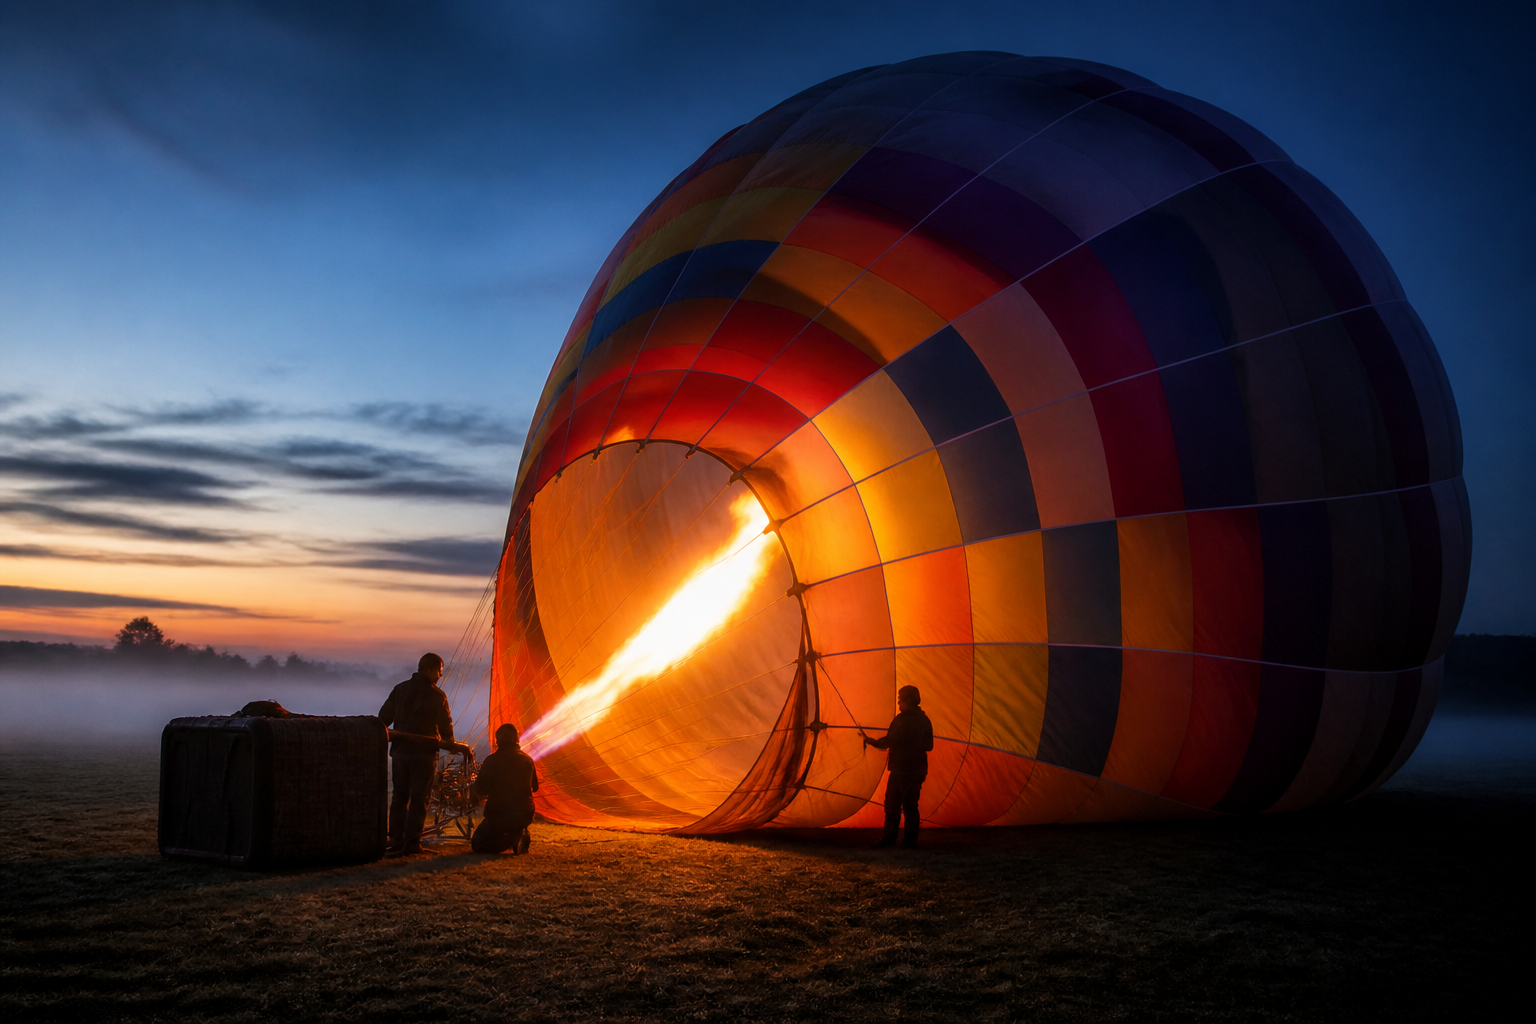
\includegraphics[width=0.58\linewidth]{images/book3/ai/b3-20-hot-air-balloon-burner.png}

{\small Menggembungkan balon udara panas: udara yang dipanaskan kurang padat daripada udara dingin di sekitarnya, dan \omterm{thm:b1:fluid-statics:archimedes}{gaya apung} Archimedes pada selubungnya melampaui beratnya.}
\end{omfigure}

\section{Soal: Kapal selam}

\begin{problem}[{Soal akhir pekan --- sebuah lambung baja tiga ratus meter
di bawah permukaan: tekanan pada pelatnya, air yang harus ditelannya untuk turun dan
disemburkannya untuk naik, penyelam yang meninggalkannya, dan kapal tanker yang lewat
di atasnya}]
\label{pb:b1:fluid-statics:1}
Air laut: $\rho = \qty{1025}{kg/m^3}$; air tawar \qty{1000}{kg/m^3};
$P_0 = \qty{1.013e5}{Pa}$; $g = \qty{9.81}{m/s^2}$. Lambung kapal selamnya
mengurung $V = \qty{3000}{m^3}$; dengan tangki pemberat kosong massanya
$m_0 = \qty{2800}{t}$.

\medskip
\noindent\textbf{Bagian I --- Tekanan pada lambungnya.}
\begin{enumerate}
  \item Tekanan mutlak pada \qty{300}{m}, dalam \omterm{def:b1:kinetic-theory:pressure}{pascal} dan dalam bar.
  \item Gaya pada palka bundar bergaris tengah \qty{0.80}{m} pada kedalaman itu;
        bandingkan dengan berat sebuah truk.
  \item Gaya pada satu meter persegi lambung di lunasnya bila lambungnya
        setinggi \qty{10}{m} dan puncaknya berada pada \qty{300}{m}: seberapa berbeda dari
        puncaknya?
  \item Air sedikit termampatkan ($\chi_T = \qty{4.6e-10}{Pa^{-1}}$):
        sebesar pecahan berapa air laut lebih padat pada \qty{300}{m} daripada di
        permukaan? Apakah itu berpengaruh pada tekanan yang dihitung di atas?
  \item Awak di dalamnya menghirup udara pada \qty{1}{atm}: mengapa lambungnya
        harus berupa tabung yang tebal, dan mengapa tabung lebih tahan
        daripada kotak datar?
  \item Sebuah kulit tabung tipis berjari-jari $R$ dan berdinding setebal $e$
        di bawah kelebihan tekanan luar $\Delta P$ mengemban tegangan
        tekan $\Delta P\,R/e$ pada dindingnya. Untuk $R = \qty{5.0}{m}$ dan
        $e = \qty{3.0}{cm}$ pada \qty{300}{m}, hitunglah lalu bandingkan dengan
        tegangan luluh bajanya, kira-kira \qty{600}{MPa}.
\end{enumerate}

\medskip
\noindent\textbf{Bagian II --- Menyelam dan mengapung.}
\begin{enumerate}[resume]
  \item Di permukaan dengan tangki kosong, berapa volume lambungnya yang muncul?
  \item Berapa massa air laut yang harus dimasukkan tangki pemberatnya agar
        kapal selamnya melayang (keterapungan netral)?
  \item Setelah melayang pada \qty{300}{m}, lambungnya termampatkan sebesar
        $0.1\%$ oleh tekanannya. Hitunglah gaya total yang timbul lalu katakan
        apakah kesetimbangannya mantap terhadap kedalaman.
  \item Kapalnya berlayar dalam keadaan melayang dari laut masuk ke
        muara berair tawar. Berapa gaya totalnya? Ke mana ia bergerak, dan apa yang harus dilakukan
        awaknya?
  \item Sebuah torpedo \qty{20}{t} ditembakkan. Apa yang harus segera dilakukan sistem
        pemberatnya, dan sebesar apa?
  \item Mengapa kapal selam memakai udara mampat untuk mengosongkan tangkinya, dan
        mengapa tekanan udaranya membatasi sampai kedalaman berapa ia dapat mengosongkannya?
  \item Taksirlah volume udara pada \qty{1}{atm} yang diperlukan untuk mengosongkan
        \qty{275}{m^3} tangki pada \qty{300}{m} (hukum Boyle, $PV$
        tetap).
\end{enumerate}

\medskip
\noindent\textbf{Bagian III --- Penyelamnya.}
Seorang penyelam meninggalkan permukaan dengan \qty{6.0}{L} udara di paru-parunya.
\begin{enumerate}[resume]
  \item Tekanan mutlak pada \qty{10}{m} dan \qty{30}{m}.
  \item Bila ia turun sambil menahan napas, berapa volume paru-parunya pada
        \qty{30}{m}?
  \item Seorang penyelam scuba menghirup udara pada tekanan sekitarnya di \qty{30}{m}
        lalu naik sambil menahan napas: berapa volume yang akan dituntut
        paru-parunya di permukaan, dan apa pelajarannya.
  \item Sebuah snorkel sepanjang \qty{1.0}{m}: berapa beda tekanan antara
        air pada dada penyelamnya dan udara di paru-parunya; berapa gaya pada
        dada seluas \qty{0.05}{m^2}; dapatkah ia menarik napas?
  \item Tabung udaranya memuat \qty{12}{L} pada \qty{200}{bar}: berapa liter
        udara pada \qty{30}{m} yang dihasilkannya, dan cukup untuk berapa lama pada
        \qty{20}{L} tiap menit?
\end{enumerate}

\medskip
\noindent\textbf{Bagian IV --- Kapal tanker di atasnya.}
\begin{enumerate}[resume]
  \item Sebuah kapal tanker \qty{100000}{t} terapung di air laut: berapa volume air
        yang didesaknya.
  \item Luas bidang airnya \qty{8000}{m^2}: sebesar apa ia naik atau
        turun ketika ia masuk ke air tawar?
  \item Memuat \qty{10000}{t} minyak: berapa perubahan saratnya.
  \item Kapal tanker yang kosong berpusat massa tinggi; ia mengangkut air laut
        sebagai pemberat ketika kosong. Mengapa, ditinjau dari metasentrumnya?
  \item Lambung kapal tankernya di lunasnya (sarat \qty{20}{m}): berapa tekanan dan
        gayanya tiap meter persegi, dibandingkan dengan kapal selam pada
        \qty{300}{m}.
  \item Kapal tankernya lewat tepat di atas kapal selamnya. Apakah kapal
        selamnya merasakan \qty{100000}{t}-nya? Jelaskan dengan medan
        tekanannya.
  \item Ringkaslah: satu hubungan yang menetapkan setiap angka dalam
        soal ini, dan teorema yang menyusul darinya.
\end{enumerate}
\end{problem}
